% !TEX encoding = UTF-8 Unicode
% !TEX TS-program = xelatex

\documentclass{article}
	\usepackage{fontspec}
	\setmainfont{SourceCodePro-Regular}
	\usepackage{tikz}
	\usepackage{listings}
\begin{document}

	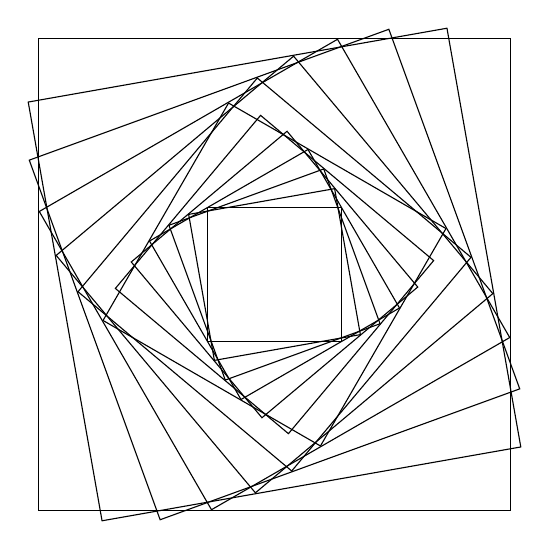
\begin{tikzpicture}
		\draw (-3, -3) rectangle (3, 3);
		\draw [scale = 0.9, rotate = 10] (-3, -3) rectangle (3, 3);
		\draw [scale = 0.9^2, rotate = 20] (-3, -3) rectangle (3, 3);
		\draw [scale = 0.9^3, rotate = 30] (-3, -3) rectangle (3, 3);
		\draw [scale = 0.9^4, rotate = 40] (-3, -3) rectangle (3, 3);
		\draw [scale = 0.9^5, rotate = 50] (-3, -3) rectangle (3, 3);
		\draw [scale = 0.9^6, rotate = 60] (-3, -3) rectangle (3, 3);
		\draw [scale = 0.9^7, rotate = 50] (-3, -3) rectangle (3, 3);
		\draw [scale = 0.9^8, rotate = 40] (-3, -3) rectangle (3, 3);
		\draw [scale = 0.9^9, rotate = 30] (-3, -3) rectangle (3, 3);
		\draw [scale = 0.9^10, rotate = 20] (-3, -3) rectangle (3, 3);
		\draw [scale = 0.9^11, rotate = 10] (-3, -3) rectangle (3, 3);
		\draw [scale = 0.9^12] (-3, -3) rectangle (3, 3);
	\end{tikzpicture}

\lstset{language=[latex]tex,tabsize=4}
\lstset{moretexcs={draw}}



%%%%%%%%%%%%%%%%%%
\begin{lstlisting}
% !TEX encoding = UTF-8 Unicode
% !TEX TS-program = pdflatex
\documentclass{article}
	\usepackage{tikz}
\begin{document}
	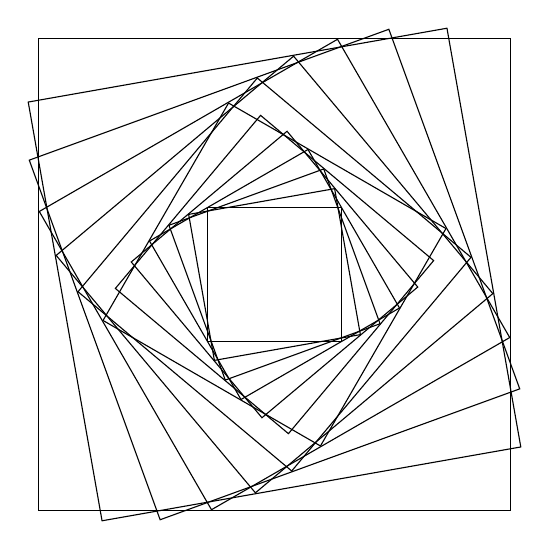
\begin{tikzpicture}
		\draw (-3, -3) rectangle (3, 3);
		\draw [scale = 0.9, rotate = 10] (-3, -3) rectangle (3, 3);
		\draw [scale = 0.9^2, rotate = 20] (-3, -3) rectangle (3, 3);
		\draw [scale = 0.9^3, rotate = 30] (-3, -3) rectangle (3, 3);
		\draw [scale = 0.9^4, rotate = 40] (-3, -3) rectangle (3, 3);
		\draw [scale = 0.9^5, rotate = 50] (-3, -3) rectangle (3, 3);
		\draw [scale = 0.9^6, rotate = 60] (-3, -3) rectangle (3, 3);
		\draw [scale = 0.9^7, rotate = 50] (-3, -3) rectangle (3, 3);
		\draw [scale = 0.9^8, rotate = 40] (-3, -3) rectangle (3, 3);
		\draw [scale = 0.9^9, rotate = 30] (-3, -3) rectangle (3, 3);
		\draw [scale = 0.9^10, rotate = 20] (-3, -3) rectangle (3, 3);
		\draw [scale = 0.9^11, rotate = 10] (-3, -3) rectangle (3, 3);
		\draw [scale = 0.9^12] (-3, -3) rectangle (3, 3);
	\end{tikzpicture}
\end{document}
\end{lstlisting}
%%%%%%%%%%%%%%%%



\end{document}